\chapter{Implementation}
\label{implementation}

MCRP is implemented on the TelosB mote platform. It uses Contiki, a lightweight operating system as the software development platform that supports the standard IPv6. The implementations of MCRP across the layers in Contiki are described in details, specifying the changes that were introduced and undertaken in addition to the default parameters and settings in Contiki.

%Contiki is a lightweight operating system with support for dynamic loading and replacement of individual programs and services. The purpose of the Contiki design is to reduce size and complexity, as well as to preserve flexibility. A running Contiki system consists of the kernel, libraries, the program loader and a set of processes (may be either an application program or a service - functionality used by more than one application process e.g. includes communication protocol stacks, sensor device drivers) \cite{contiki}. 
 
%\section{Contiki Protocol Stack (changes at MAC, RT, NBR TB, BR etc.)}
\section{Contiki}
%MCRP is a cross layer protocol implemented on Contiki version 2.7. (explain what is cross layer? why do cross layer? FIGURE OF STACKS)

\begin{table}
  \centering
    \begin{tabular}{|c|c|c|}
      \hline
      Contiki & IoT/IP & Applications \\
      \hline \hline
      \multirow{4}{*}{Network} 
        & Application & HTTP \\
        \cline{2-3}
        & Transport & TCP, UDP \\
        \cline{2-3}
        & Network, Routing & IPv6, IPv4, RPL \\
        \cline{2-3}
        & Adaptation & 6LoWPAN \\
      \hline \hline
      
      MAC & MAC & CSMA/CA \\
      \hline
      RDC & Duty Cycling & ContikiMAC \\
      \hline
      Radio & Radio & IEEE 802.15.4 \\
      \hline
    \end{tabular}
    \caption{Contiki network stack}
    \label{table:1}
\end{table}

Contiki is defined by four layers network stack: the network layer, the MAC layer, the radio duty cycling (RDC) layer and the radio layers. The network layer includes support for TCP, UDP, IPv6, IPv4, RPL routing protocol and 6LoWPAN. IPv6 over Low Power Wireless Personal Area Networks (6LoWPAN) is a header compression and fragmentation format for IPv6 packets delivery over IEEE 802.15.4 networks \cite{6lowpan}. Contiki implements the minimal set of IPv6 protocol required, 6LoWPAN adaptation layer for IPv6 header compression and fragmentation which is routed over the low power and lossy networks (LLN) in RPL.

Contiki's configuration options for communications, buffer management and network interface are explained below.
%before looking into MCRP implementation for ease of reading.

%6LoWPAN working group specified header compression and fragmentation for IPv6 over IEEE 802.15.4 (///REFERENCE!!!) and the IETF RoLL working group designed the RPL protocol as a proposed standard for IPv6 routing in low-power and lossy networks (LLNs). Contiki implement the necessary parts of the IPv6 protocol, IPv6 header compression and fragmentation with the 6LoWPAN adaptation layer, routing over LLNs with the RPL protocol, as well as a set of protocols from the TCP/IP protocol suite \cite{beyondInteroperability}.

%///RPL does not rely on any particular features of a specific link-layer technology.  RPL is designed to be able to operate over a variety of different link layers, including ones that are constrained, potentially lossy, or typically utilized in conjunction with highly constrained host or router devices, such as but not limited to, low-power wireless or PLC (Power Line Communication) technologies.\cite{winter2012rpl}

\subsection{Communication Stacks}
\label{commstack}
Contiki contains two communication stacks, uIP and Rime.
uIP \cite{uip} is a small RFC-compliant TCP/IP stack that is designed to contain only the essential features to provide Contiki with TCP/IP networking support to allow Contiki to communicate over the Internet compared to the traditional TCP/IP that requires (high) resources to fit in a limited RAM capabilities of a sensor. The minimal set of features includes IP, ICMP, UDP and TCP protocols compared to the traditional TCP/IP that requires resources that could not be supported in the limited RAM capabilities sensor. The uIP deals with the TCP and IP protocols \cite{contikiDoc, contikiUIP}. 

Rime is Contiki's lightweight communication stack that aims to simplify the sensor network protocols implementation by reusing code in a layered manner \cite{rimeposter}. Rime combines layers of simple communication abstractions to form a powerful high-level abstraction ranging from best-effort anonymous broadcast to reliable network flooding. Parts of the Rime stack can be used by the underlying MAC or link layer. Additional protocols that are not in Rime can be implemented on top of the stack.

Applications in Contiki can decide to use one of the communication stacks available, both or none at all. uIP can run over Rime and similarly, Rime can run over uIP \cite{contikitutorial}. This allows protocols or applications that are not in Rime or uIP to be implemented directly on top of the communication stack such as running TCP/IP on Rime.

%Rime communication stack provides a set of lightweight communication primitives ranging from best-effort anonymous local area broadcast to reliable network flooding. Protocols or applications running on top of Rime stack can implement additional protocols that are not in the Rime stack such as TCP/IP.

%Rime draws heavily from communication abstractions for distributed programming.

%draws heavily from communication abstractions for distributed programming where layers of simple abstractions are combined to form powerful high-level abstraction. The purpose of Rime is to simplify implementation of sensor network protocols and facilitate code reuse. The thin layers in Rime enable code reuse within the stack. An underlying MAC or link layer may chose to implement parts of the Rime stack \cite{rimeposter}. 

%Traditional TCP/IP implementations have required far too much resources which is impossible to fit in a sensor that has limited RAM capabilities (RAM is the most scarce resource). uIP \cite{uip} is a small RFC-compliant TCP/IP stack that makes it possible for Contiki to communicate over the Internet. uIP implementation is designed to have only the absolute minimal set of features needed for a full TCP/IP stack such as IP, ICMP, UDP and TCP protocols. The uIP is mostly concerned with the TCP and IP protocols and upper layer protocols \cite{contikiDoc, contikiUIP}. 

\subsection{Buffer Management}
\label{bufmgmt}
Chameleon \cite{rime} is a communication architecture in Contiki that consists of Rime communication stack and a set of packet transformation modules. It uses an abstract representation of the information which allows access to the low-level features of the underlying MAC and link layer protocol from the applications and layers implemented on top of the Chameleon architecture. It also allows the output from the protocol stack to be adapted by other communication protocols. In Chameleon architecture, the parsing of its header is separated from the communication stack. This allows uIP or Rime communication stack to be used as described in Section \ref{commstack}. Chameleon architecture enables the layers to access information without violating the layering principle. 

%other communication protocols such as link and MAC layer protocols and TCP/IP. -input output?

%It allows access to the features of underlying MAC and link layer protocols for the implemented protocols on top of the architecture. 

%The use of packet attributes makes it possible to adapt the output from the protocol stack to other communication protocols such as link and MAC layer protocols and TCP/IP.

%Chameleon is a header construction. The parsing is done separately from the communication stack which allows the use of uIP or Rime communication stack that both are supported in Contiki.

%\cite{rime} introduces Chameleon, a communication architecture for sensor networks consists of Rime communication stack and a set of packet transformation modules. Rime communication stack provides a set of lightweight communication primitives ranging from best-effort anonymous local area broadcast to reliable network flooding. Protocols or applications running on top of Rime stack can implement additional protocols that are not in the Rime stack such as TCP/IP.

%Chameleon does not define any packet headers but instead uses $packet attributes$, an abstract representation of the information usually found in packet headers to allow applications to access low-level information without violating the layering principle. Packet headers are produced by separate header transformation modules that transform application data and packet attributes into packets with header and payload. The use of packet attributes makes it possible to adapt the output from the protocol stack to other communication protocols such as link and MAC layer protocols and TCP/IP.
%Chameleon architecture allows for sensor network protocols that are implemented on top of the architecture to take advantage of the features of underlying MAC and link layer protocols.

In buffer management module of Chameleon architecture, all incoming and outgoing packets from the applications and packet attributes are stored in a single buffer called the Rime buffer \cite{uip, rime, rimeposter, contiki}. All layers of Contiki's network stack including uIP, Rime and the underlying link layer operate on the same packet buffer for the buffer management. The Rime buffer has no locking mechanisms as it is a single priority level buffer. The buffer only holds the current packet.

Protocols that need to queue packets allocate the queue buffer dynamically. Queue buffer is used to hold the queued packets such as for MAC protocols that have high rate of incoming and outgoing messages before it can send or process the receiving packets; or when the radio is busy and the MAC protocol has to wait for the radio medium to be free before proceeding with transmissions. 
%Queue buffer is used to avoid the risk of the packet overwritten by the newer packet. 
The Rime buffer contents are copied into the queue buffer when there is a queue buffer allocated.

%Protocols that need to queue packets, such as MAC protocols that wait for the radio medium to be free, can allocate so-called queue buffers to hold the queued packet. Queue buffers are dynamically allocated from a pool of queue buffers. The contents of the Rime buffer, including the packet attributes, are copied into the queue buffer when it is allocated.

%All layers of the netstack operate on the packet buffer. 
%Rime's buffer management module is used by the underlying link layer for buffer management.
%The packet buffer only holds the current packet.

%Even though it is called a Rime buffer, both uIP and Rime uses the same buffer.

%In the buffer management of Chameleon architecture, all packets both outgoing and incoming are stored in a single buffer \cite{rimeposter}, called the Rime buffer. 
%The Rime buffer contains both the application data and the packet attributes. All access to the Rime buffer is done at a single priority level so no locking mechanisms need to be used.

%Rime's buffer management module is used by the underlying link layer for buffer management.
%////BUFFER MANAGEMENT - since it's related to uIP (Chameleon, Rime etc)

%All layers of the netstack operate on the packet buffer. One buffer holds a single packet. ***Uses a single buffer for both incoming and outgoing packets \cite{uip, rime, rimeposter, contiki}. The packet buffer only holds the current packet.

%Buffer for uIP and Rime is the same. They use the same buffer.
%\subsection{Retransmission} 


%It uses (EXPLAIN CONTIKIMAC - refer to contikimac paper; why it's good, how it works). Also about retransmission and buffers. (maybe at next section???) The transmitting channel is set at the MAC layer as packets are not send immediately if there are packets being queued. The channel is reset to the transmitting channel before it tries to send and it is then reset to the listening channel to wait and listen to any packets that is being sent to the node. 

%The default ContikiMAC is a single channel protocol. It is modified to be able to work with multi channel nodes while (stick/hold/is) on the same principle of a low power ContikiMAC (minor changes to support multi channel without changing the main purpose of ContikiMAC).

\subsection{Tunslip}
Serial Line Internet Protocol (SLIP) \cite{slip} is a protocol that has a low complexity and small overhead commonly used to encapsulate IP packets for point-to-point communication between the sink (LPBR) and the device connected such as an embedded PC across the serial connections. The communication between the devices can take place on any reliable network such as the Ethernet where the LPBR can be connected to an embedded PC which contains an Ethernet interface.
%which the interface is available in the embedded PC.

%Serial Line Internet Protocol (SLIP) //need reference!!!] is used for the communication between the sink and the device which it connected to such as an embedded PC. 
%SLIP is commonly used to encapsulate IP packets for transmission across the serial line of micro-controller devices. 
%SLIP has a low complexity and small overhead. 
%For the communication between the devices (embedded PCs), any reliable network can be used (e.g. Ethernet). 
%The sinks are connected to an embedded PC which contains an Ethernet interface. The communication between the sink (sensor node) and the embedded PC makes use of SLIP. 

Contiki provides support to communicate with devices using SLIP through its tunslip tool. Tunslip is used to bridge the IP traffic between the LPBR and the embedded PC over a serial line. The other side of the serial line does a similar job to bridge the embedded PC to the LPBR using the network interface. It constructs a SLIP tunnel between a virtual network interface (tun) and SLIP, the physical serial interface to encapsulate and pass the IP traffic to and from the other side of the serial line. The tun interface is used as any real network interface such as for routing and traffic forwarding \cite{tunslip, multipleSinks}.

%Contiki already provides support for SLIP communication and includes a tunslip tool (need reference!!!) which make it possible to communicate with devices using SLIP. 
%The tool constructs a SLIP tunnel between a physical serial interface and a virtual network adaptor. 
%By using tunslip the communication between the sink and the embedded PC is facilitated \cite{multipleSinks}.

%Tunslip is a too used to bridge IP traffic between a host and another network element, typically a border router, over a serial line. 
%Tunslip creates a virtual network interface (tun) on the host side and uses SLIP (serial line internet protocol) to encapsulate and pass IP traffic to and from the other side of the serial line. 
%The network element sitting on the other side of the line does a similar job with it's network interface. 
%The tun interface can be used like any real network interface: routing, traffic forwarding etc \cite{tunslip}.


\section{MCRP Implementation}
MCRP is implemented in Contiki and uses ContikiMAC as the MAC protocol and RPL as the routing protocol. ContikiMAC is modified to allow multichannel where the channel selection processes take place on the upper layers and the channels are kept in the network neighbour table to ensure the correct channel.

The protocol implementation is separated into two types of nodes: i) the centralised LPBR where the bridging takes place between the border router on a PC to the nodes, and ii) the decentralised transmission nodes referred as other nodes. The implementations for both types are described below.

%MCRP is implemented as an extension to the existing implementation of RPL with ContikiMAC; to enable multi channel.
%The protocol is implemented by tailoring existing code of ContikiMAC, network layer and RPL.

%\subsection{Application Layer}
%//separate into 2; setCh and xSetCh as LPBR is separated with BR and SR
%//access Network layer - Neighbour table, set channel

\subsection{Low Power Border Router}

\begin{figure}
\centering
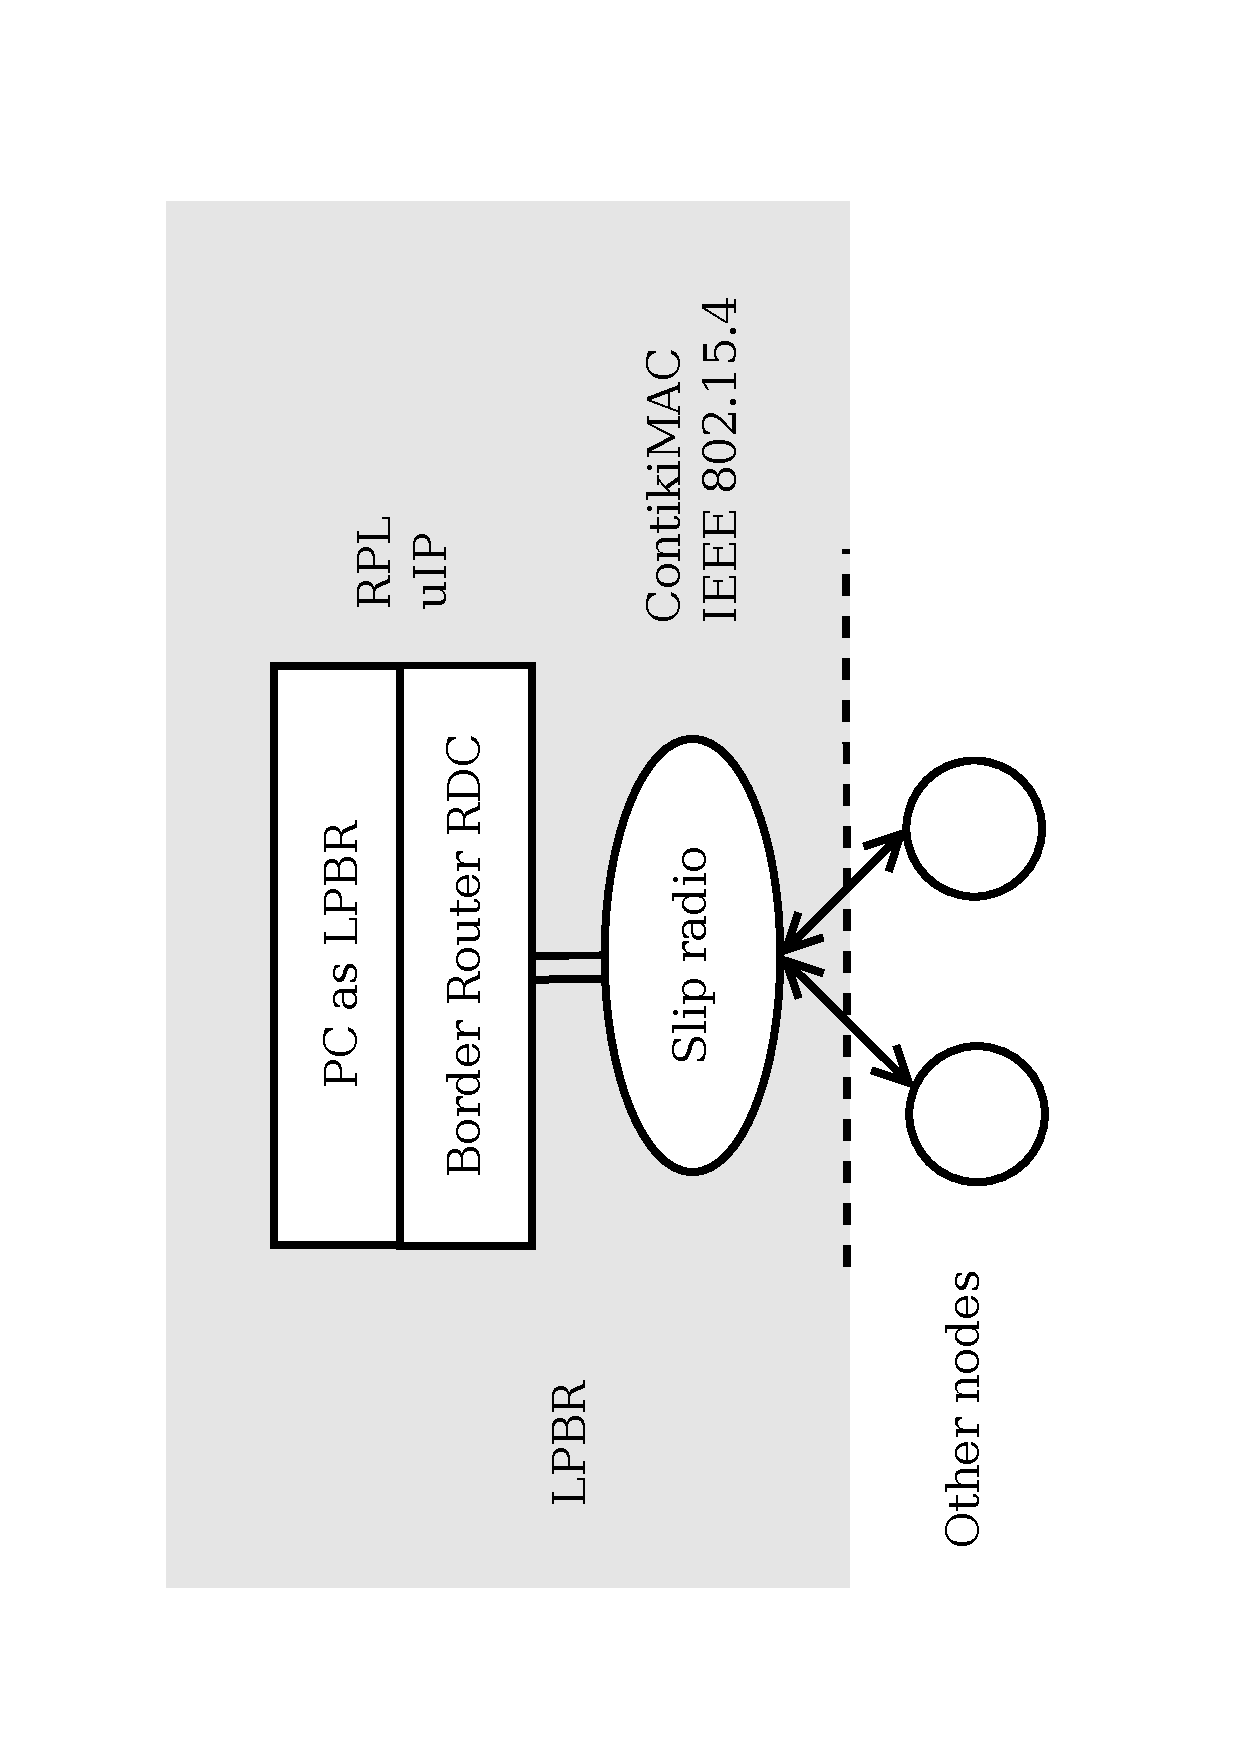
\includegraphics[trim=2cm 2cm 3cm 2cm, clip=true, totalheight=0.45\textheight, angle=270]{BR2.pdf}
\caption{Low power border router}
\label{fig_lpbr}
\end{figure}

As sensors have limited memory, most processing decisions at LPBR are transferred to a PC as it has more RAM and better processing capabilities. This enables MCRP to perform more complex processing and to run in real time without draining the memory and battery on a sensor. The LPBR is divided into two main parts as shown in Figure \ref{fig_lpbr} where the PC is responsible as the application, transport, network and routing layers while a sensor (labelled slip radio) is set as the wireless interface to enable the PC to communicate with the other nodes via the Contiki tunslip tool. 

The LPBR acts as the tree root in RPL where it will initiate the creation of the RPL routing tree. LPBR is a special case as channel changes at LPBR is not as direct as other sensor nodes due to these two parts. However, it works similar ways to the other nodes.

%It (tunslip6) sets up an interface on the Linux IP stack and connects this interface via a socket to the border router node.
%Border router is used to bridge the wireless IPv6 network to a PC via serial link which enables the IPv6 network traffic to reach outside network and the Internet.
%A node is used as a wireless interface (IEEE 802.15.4 to enable the serial socket server), a host machine as border router to bridge the wireless IPv6 network to outside network and the Internet.

%trim top left

The LPBR main responsibility is to decide on the new channel selection. The LPBR has no knowledge of all the channels condition at this point, thus, a channel is selected at random. The LPBR keeps the results from the channel changes processes and based on it when selecting a new channel for the next node to ensure the new channel is at least two-hop away from another node using the same channel. This is done to ensure that the nearby nodes do not communicate on the same channel and risk interfering with each other.

\begin{algorithm}
\caption{Pseudo-code for two-hop colouring algorithm}
\label{twohop_algo}
\begin{algorithmic}[]
\\\textbf{Notations}
\\$R$ is a node that is a Route
\\$N$ is a node Neighbour
\\$RN$ is the Route's Neighbour node
\\$currentCh$ is the node current listening channel
\\$newCh$ is the new channel the node will change to
%\\$rnCh$ is the route's neighbour channel
\\\textbf{Pseudo-code}
\\Check if there are nodes which need a new channel
\\Generate a $newCh$ by random
%\If{$R$ $=$ $R$ in $LPBR$ $nodesTable$}
%	\State check $R$ $currentCh$
	\If{$R$ $currentCh$ $\neq$ $newCh$}
		\State succeed one-hop
		\State check all $RN$ channels
		\If{$RN$ channel $\neq$ $newCh$}
			\State succeed two-hop
			\State confirm $newCh$
		\EndIf
	\Else
		\State generate a new $newCh$
		\State update the number of $newCh$ generated for $R$
			\If{number of $newCh$ generated $>$ 3}
			\State use default channel 26 is all tries fail
			\EndIf
	\EndIf
%\EndIf
\end{algorithmic}
\end{algorithm}

The pseudo-code of the implemented two-hops colouring algorithm for new channel selection is shown in Algorithm \ref{twohop_algo}. When the new channel is selected, LPBR will send the value to the intended node.

%/////RPL border router is used as LPBR in order to move most processing decisions on a PC as it has more RAM and better processing capabilities than a sensor. (Explain BR-SR how it works!)
%TelosB has limited RAM and ROM of 10K bytes and 48K bytes of flash memory \cite{telosb-datasheet}. By using a border router, this allows channel changing to be decided in real time without draining the memory and battery on a sensor. The border router also acts as the root of the tree. The border router will setup the IPv6 prefix of the network and will initiate the creation of the RPL routing tree.
%It (tunslip6) sets up an interface on the Linux IP stack and connects this interface via a socket to the border router node.
%Border router is used to bridge the wireless IPv6 network to a PC via serial link which enables the IPv6 network traffic to reach outside network and the Internet.
%A node is used as a wireless interface (IEEE 802.15.4 to enable the serial socket server), a host machine as border router to bridge the wireless IPv6 network to outside network and the Internet./////

%\begin{figure}
%\centering
%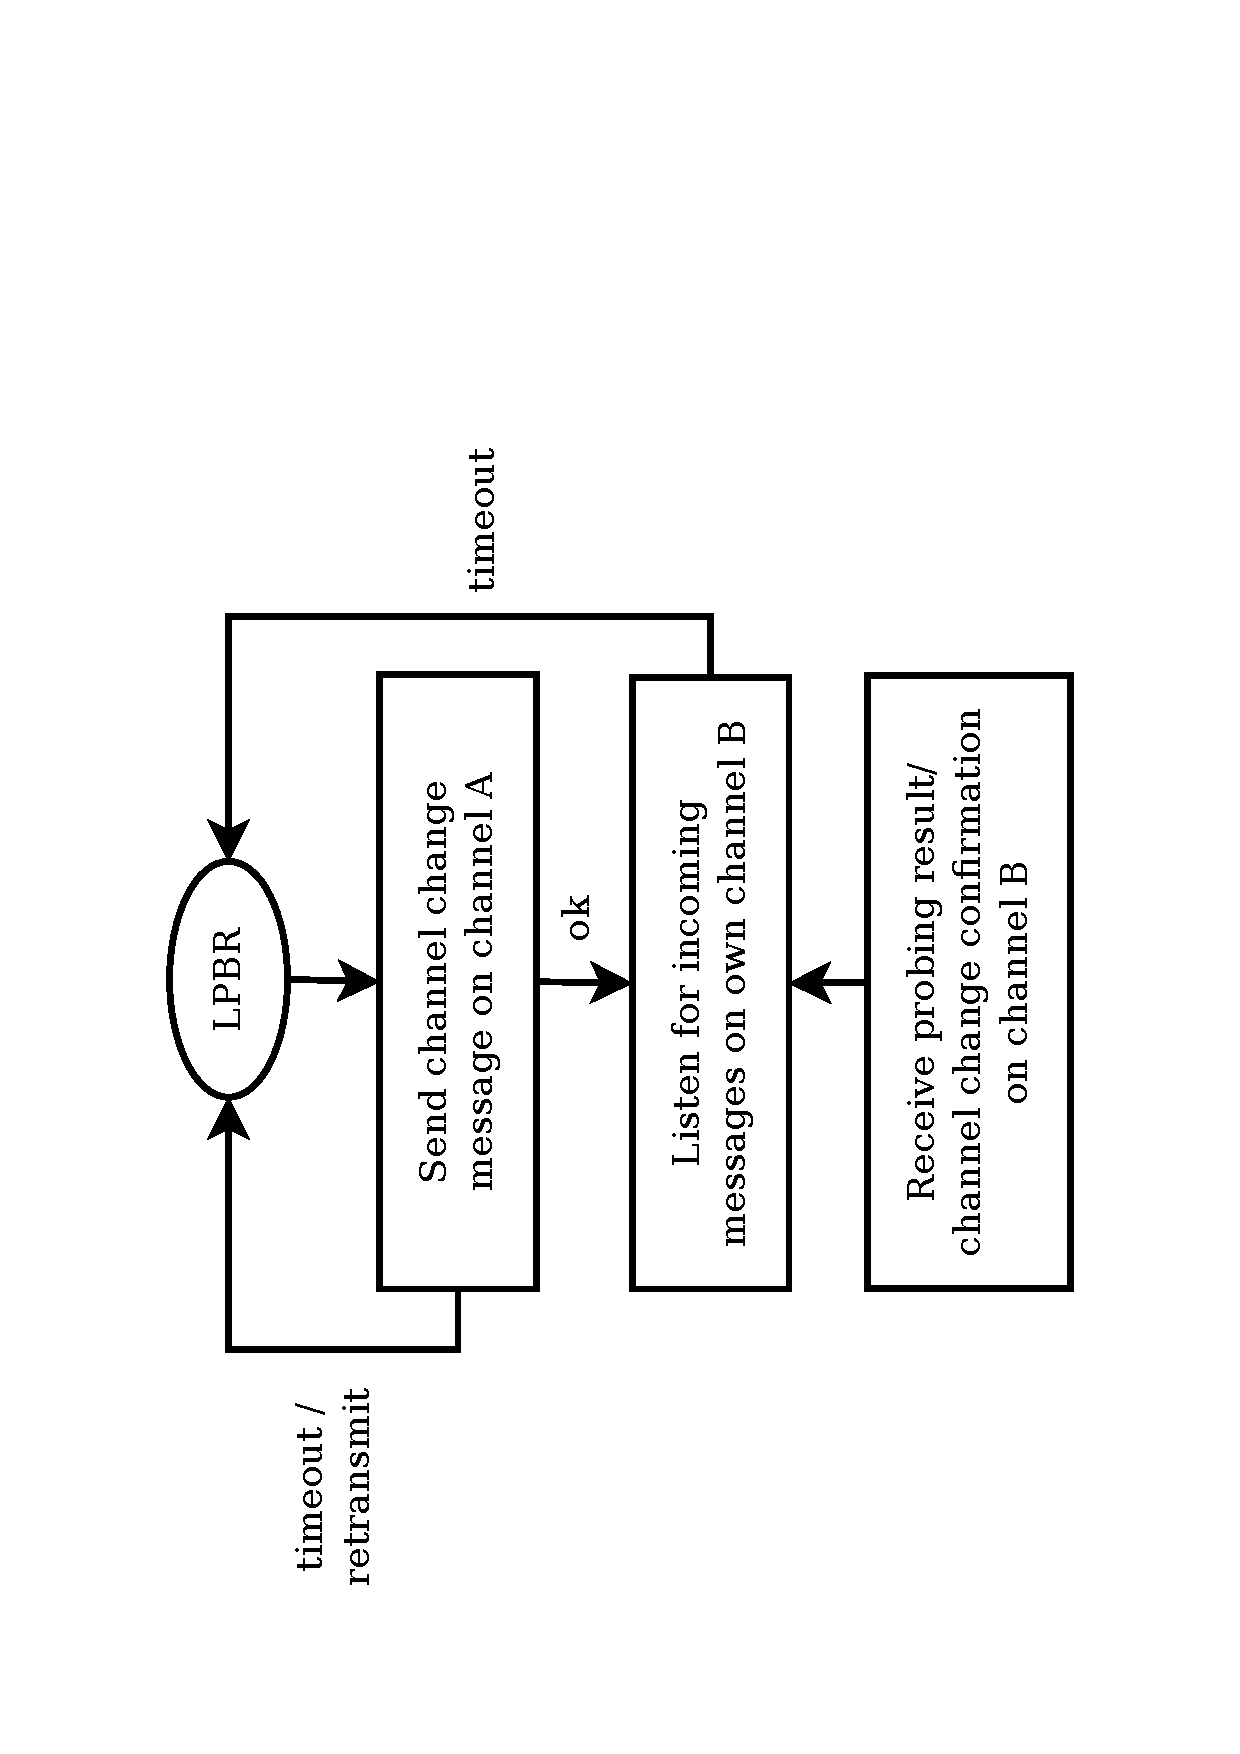
\includegraphics[trim=2cm 1cm 2cm 4cm, clip=true, totalheight=0.55\textheight, angle=270]{lpbrProcess.pdf}
%\caption{LPBR processes}
%\label{lpbrProcess}
%\end{figure}
%top, left, bottom, right

The new channel is stored in the buffer before the data is sent over SLIP to the radio-chip (slip-radio). As the slip radio is unable to access the neighbour table where the next hop node channel is stored, the channel value is passed through the buffer. LPBR keeps the updated value of all its neighbours channels in the neighbour channel. Slip radio that receives the packet buffer can access the channel value and kept the value is a simplified version of the neighbour table. This is done in order to ensure that the packet that is being queued or retransmitted is sent on the correct channel. The packets destination, which in this case, the next hop node is first check before the packet is transmitted each time. The MAC layer sets the channel accordingly before sending. ContikiMAC can access the simplified neighbour table as it is on the slip radio. The simplified neighbour table only keeps the information of the node neighbours and neighbours channels which are the critical information in order to transmit packets correctly. The other information that is related to the neighbours' conditions is monitored at the PC. 

%LPBR processes are shown in Figure \ref{lpbrProcess}.
The slip-radio resets to its listening channel after the packet is transmitted. LPBR will wait and listen to any incoming packets. In the channel probing phase, LPBR does not take part in probing. However, LPBR is informed of the results of probing and kept a table of the probing results and channels to be able to use the information when deciding on a channel change based on the previous results of probing on the known channels.

%Before passing to slip-radio, the header from $uip\_buf$ is compress to $packetbuf$. From $packetbuf$ to $uip\_buf$ is it decompress to access the data from the upper layers.  

%-send to BR RDC, check nbr table for the currentCh. pass the value to s-r. save the chvalue in a simplified nbr table to allow retx/queue to send on correct ch.
%MAC set the channel accordingly before sending.
%Change to its listening channel after finish sending. 

\subsection{Other Nodes}

%\begin{figure}
%\centering
%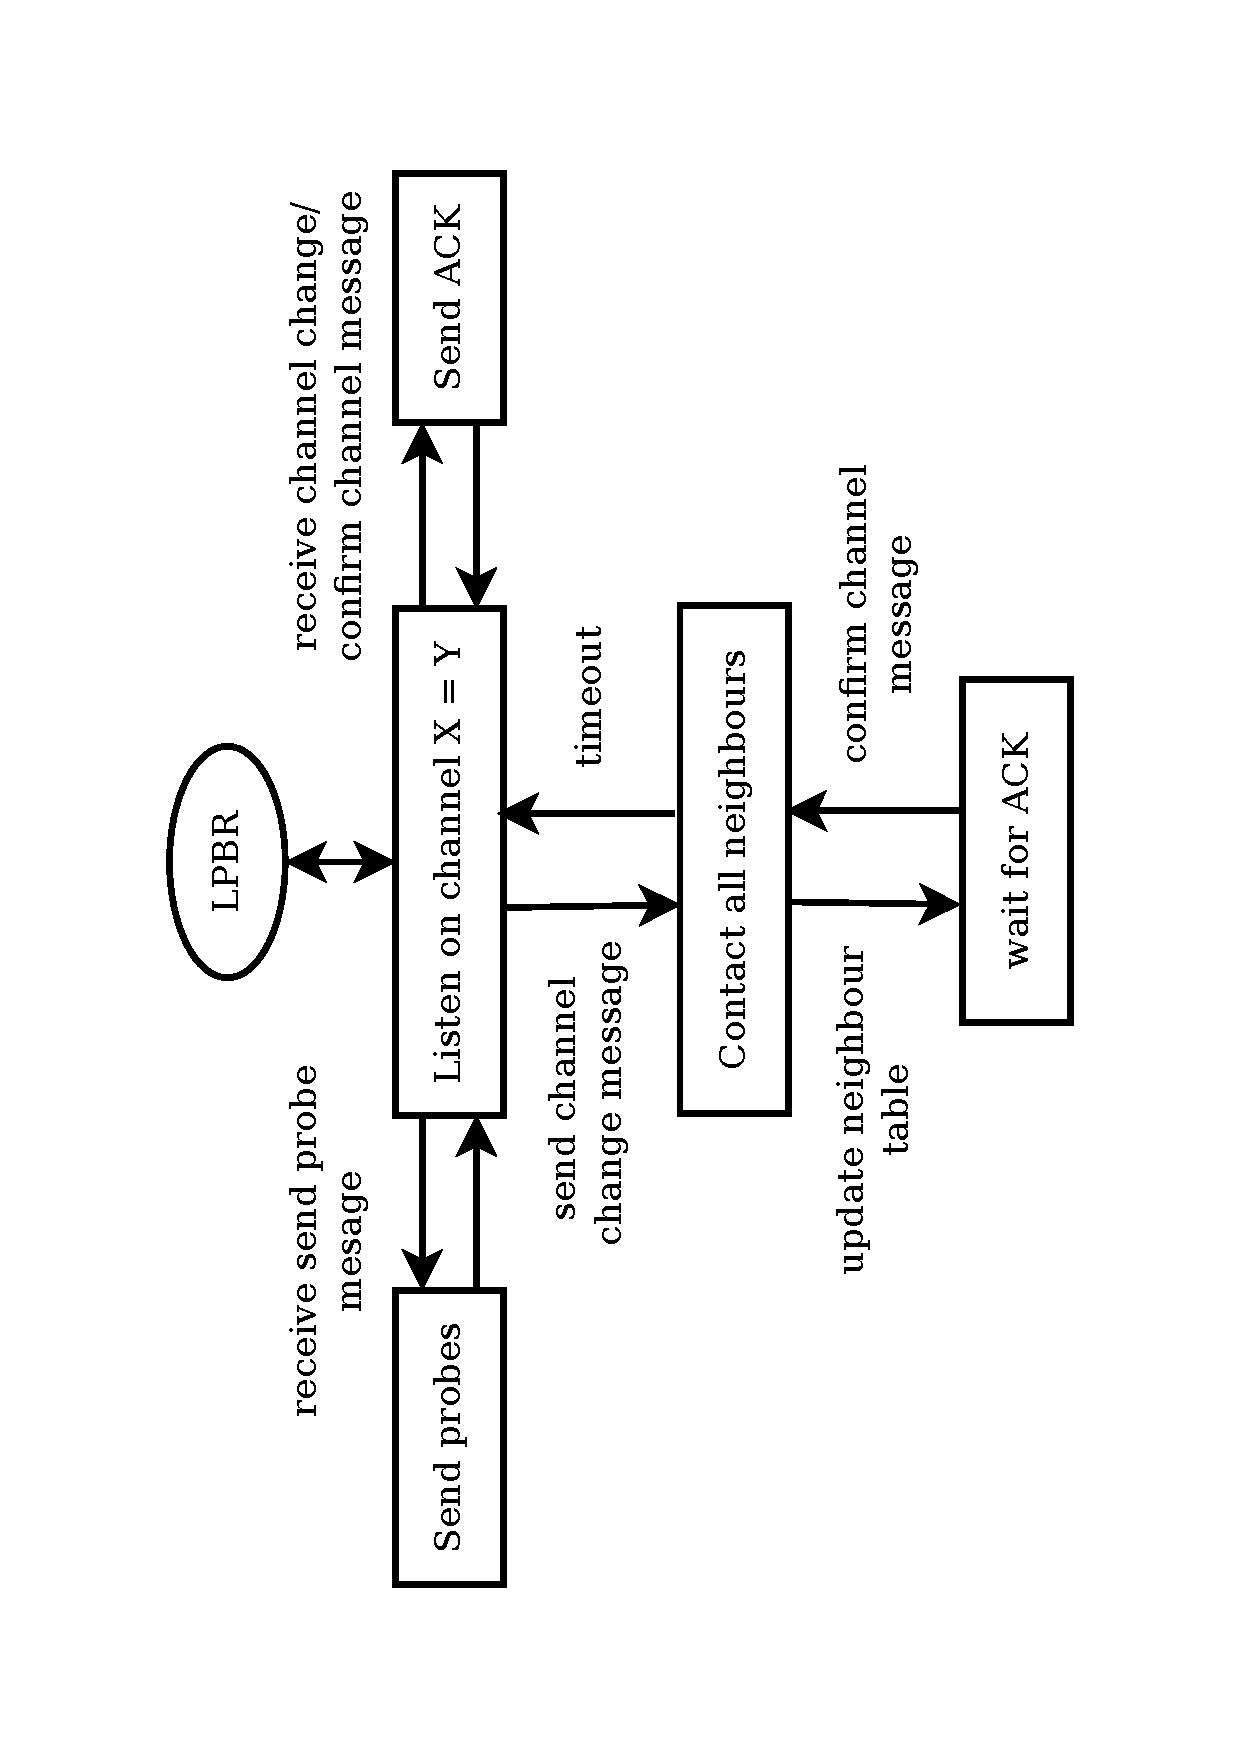
\includegraphics[trim=2cm 2cm 2.5cm 2cm, clip=true, totalheight=0.58\textheight, angle=270]{otherNodes.pdf}
%\caption{Nodes channel change processes}
%\label{fig_otherNodes}
%\end{figure}

The new channel from LPBR that is received by the destination node is saved. 
%Figure \ref{fig_otherNodes} shows the processes that the node takes in the channel change. 
When LPBR sends a \textit{Channel Change} message to the destination node, the destination node will send a packet back to LPBR to acknowledge the channel change message. If LPBR does not receive the message, the channel change message is retransmitted. LPBR will then wait and listens for any incoming packets. At this point, channel changes processes will take place between the node and its neighbours. To clarify, \textit{node} refers to the node that would like to change its listening channel and \textit{neighbour node} is the neighbour of the node (including route node) that takes part in the channel change decision through probe message.

%All nodes keep the neighbours channel in the \textit{neighbour table}. An entry is added in the neighbour table to hold the channel value called \textit{nbrCh}. 
Unlike LPBR, other nodes have all the layers within the nodes themselves. This makes channel changes less complicated, however, the nodes are being limited by the number of RAM they have which resulted in probing values to be stored in the centralised LPBR. The nodes however, keep the probing results temporarily before the final decision of the channel is made. 
%The nodes have cross-layer access. They can gain information from any layer when required.

The node sends the \textit{Node New Channel} value to all of the node's neighbours. At this point, the new channel is not yet checked for its validity. However, all neighbours need to know the new channel as the node will change its listening channel to the new channel. Otherwise, packets cannot be received by the node since the listening channel is different than it was previously. The neighbours that receive the node's channel will update their \textit{neighbour table} which is accessed from the application layer. 
Unlike LPBR, other nodes have all the layers within the nodes themselves. This makes channel changes less complicated as the nodes can access the information from any layer when required which in this case, accessing the neighbour table at the network layer from the application layer.
In the neighbour table, a new entry is added to hold the channel value called \textit{nbrCh}. As this is an important step in order to reduce the number of packet loss due to sending on the wrong channel, neighbours will send an acknowledgement of the new channel. Otherwise, it will be retransmitted. 

The node will then send a \textit{Start Probe} message to the neighbour that is a route node to start sending probing messages on the new channel. Not all neighbours are used as routes. The neighbours are chosen as route based on RPL OF which for this experiment is the ETX. The node will listens on the new channel and wait for the \textit{Neighbour Probe} message. The route node starts to \textit{Send Probe} messages every 3 seconds to allow retransmission or collision that could happen due to the busy channel. The maximum number of retransmission is configured to 3 attempts following the default value Contiki suggested. Collisions happen when the channel check keeps failing and new packets are constantly generated which could end up in a loop where no packets can be sent. The assumption that was made in this case is the channel will be cleared at some point which this loop will not happen. From the experiments and simulations, this was proved true.

%(////what is retransmission? what is collision??? how it happens? how long? collision has no time out!). 
As only a small number of \textit{Send Probe} messages are sent, the number of retransmissions and collisions that happen during the probing process are included in the channel decision process as it affects the channel reliability.
%the we are sending a small number of probe message, to increase the channel reliability of the probing, we also take into account the number of retransmission and collision that happen. 
As the retransmission and collision is a link layer process, the values are kept in a temporary \textit{Retransmit Table} and is included to be sent in the next \textit{Send Probe} message. This is because the value is only valid for that run. It gets reset each time a new packet is sent or received. The table is accessed at the application layer before the next \textit{Send Probe} message is sent. The \textit{Send Probe} message includes the current number of probe message and the number of tries (retransmissions and collisions) the previous packet had taken before it is successfully received. These values are used to decide if the channel is better than the current channel by giving a good probing result, meaning less retransmission.

The node keeps the value of all probing messages it receives. It sends the \textit{Probe Result} message to LPBR. 
Unlike LPBR, the node has a limited RAM which resulted in past probing values to be stored in the centralised LPBR. The node however, keeps the probing results temporarily before the final decision of the channel is made. 
LPBR could use the information from the node's \textit{Probe Result} to decide on a channel or blacklist bad channels. 

The node then uses the values to decide whether the new channel is better than the previous channel by setting a threshold. The node then send \textit{Confirm Channel} message to all neighbours that the node confirms to be listening on. The channel can be the new channel or the node can revert to the previous channel depending on the \textit{Probe Result}. The neighbours will send an acknowledgement back to the node confirming the change. This is also important to ensure that all neighbours could communicate with the node on the correct channel. The neighbours will update their neighbour table of the node channel. 

\subsection{MAC Layer}
%As MCRP is a cross-layer protocol, 
As explained in Section \ref{bufmgmt}, packets that have not been transmitted are queued in the buffer. The transmitting channel is set at the MAC layer as packets are not send immediately if there are packets being queued. ContikiMAC is a single channel protocol. It is modified to support multichannel while complying to the same low power ContikiMAC principle. Each time the node goes to sleep, it will wake up on its listening channel waiting for incoming packets. If the node has a packet to send, it needs to change to the transmitting channel.

In order for the packet transmission or retransmission to be on the correct channel, the neighbour channel saved in the \textit{neighbour table} at the network layer is accessed from the MAC layer and the channel is set to the transmitting channel. The node resets the channel to its listening channel after the transmission succeeded and goes back to sleep.

%\begin{figure}
%\centering
%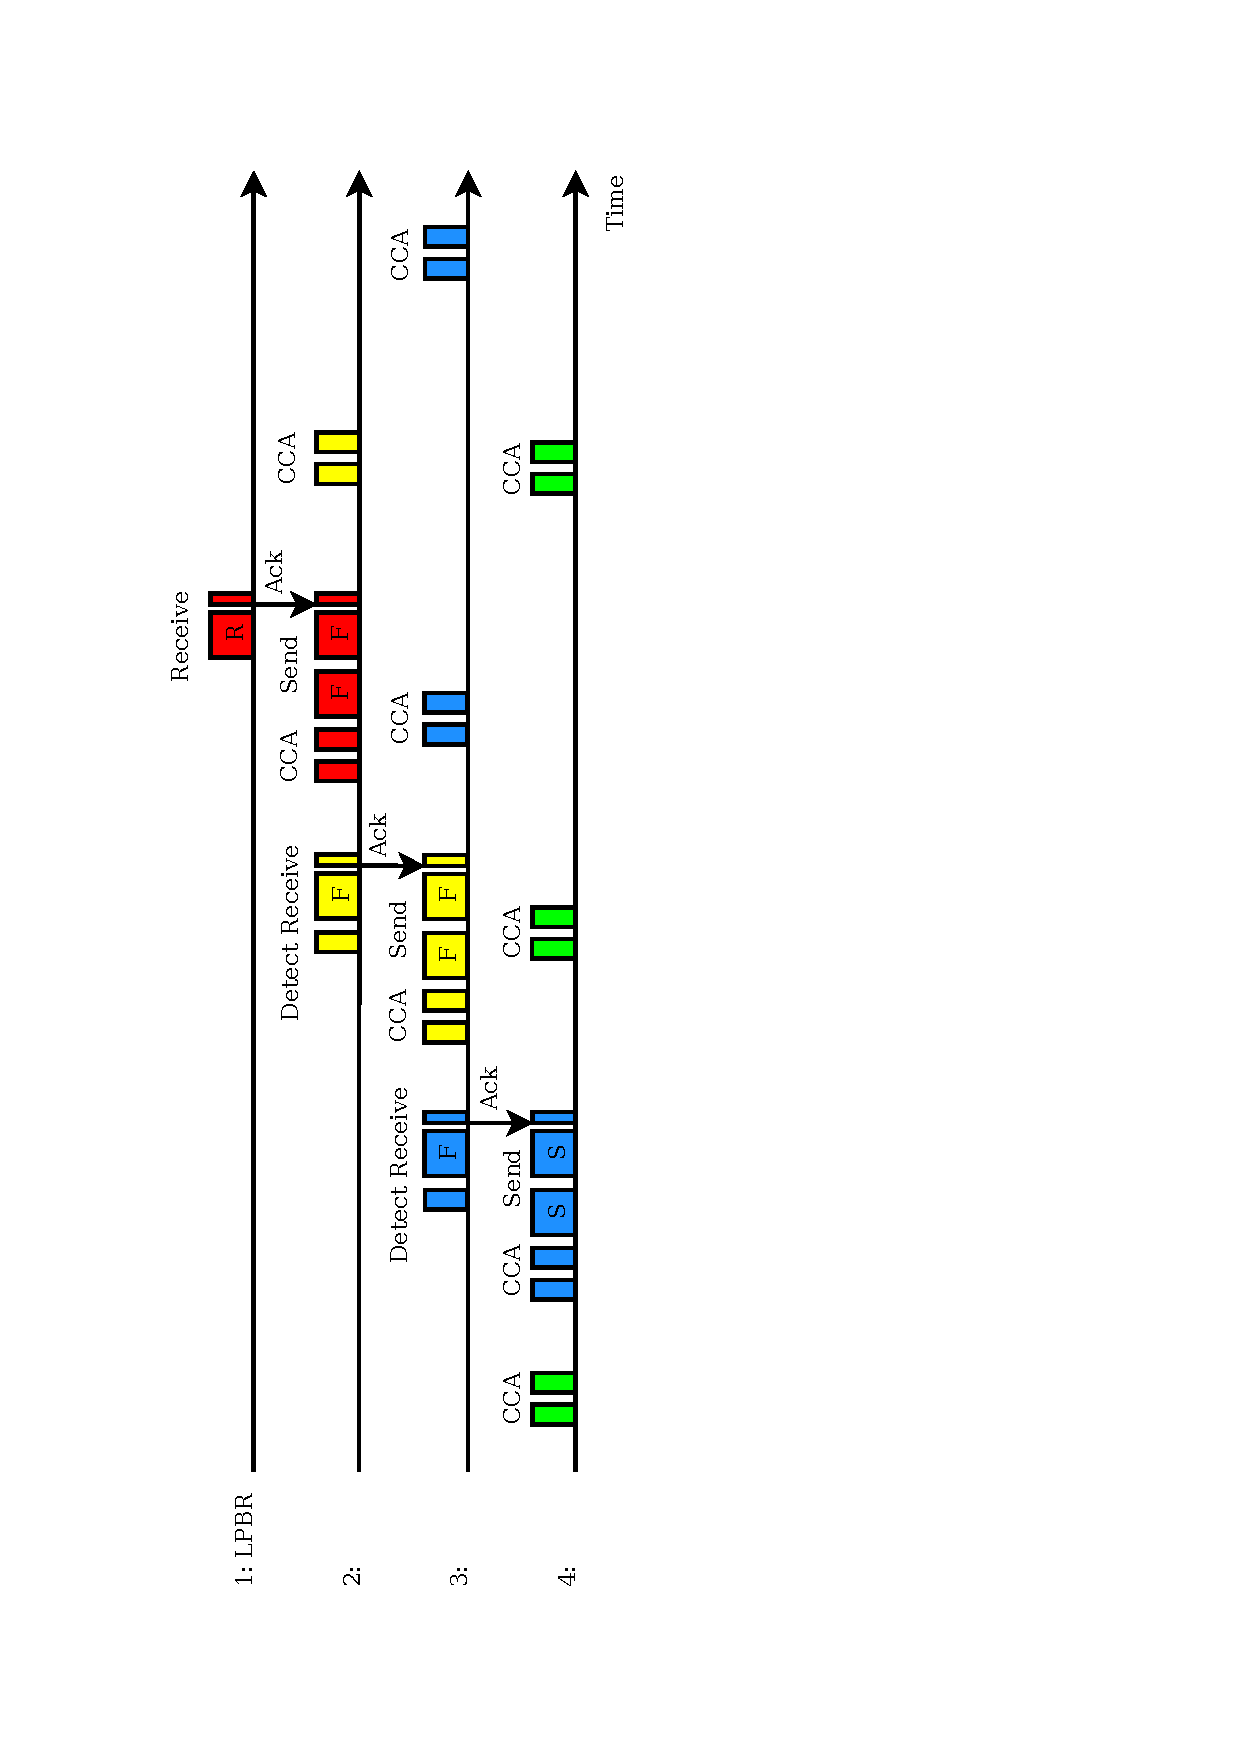
\includegraphics[trim=2cm 2cm 10cm 2cm, clip=true, totalheight=0.62\textheight, angle=270]{macExample2.pdf}
%\caption{Multi channel ContikiMAC multi hop packet transmission}
%\label{fig_mac}
%\end{figure}

%\begin{figure}
%\centering
%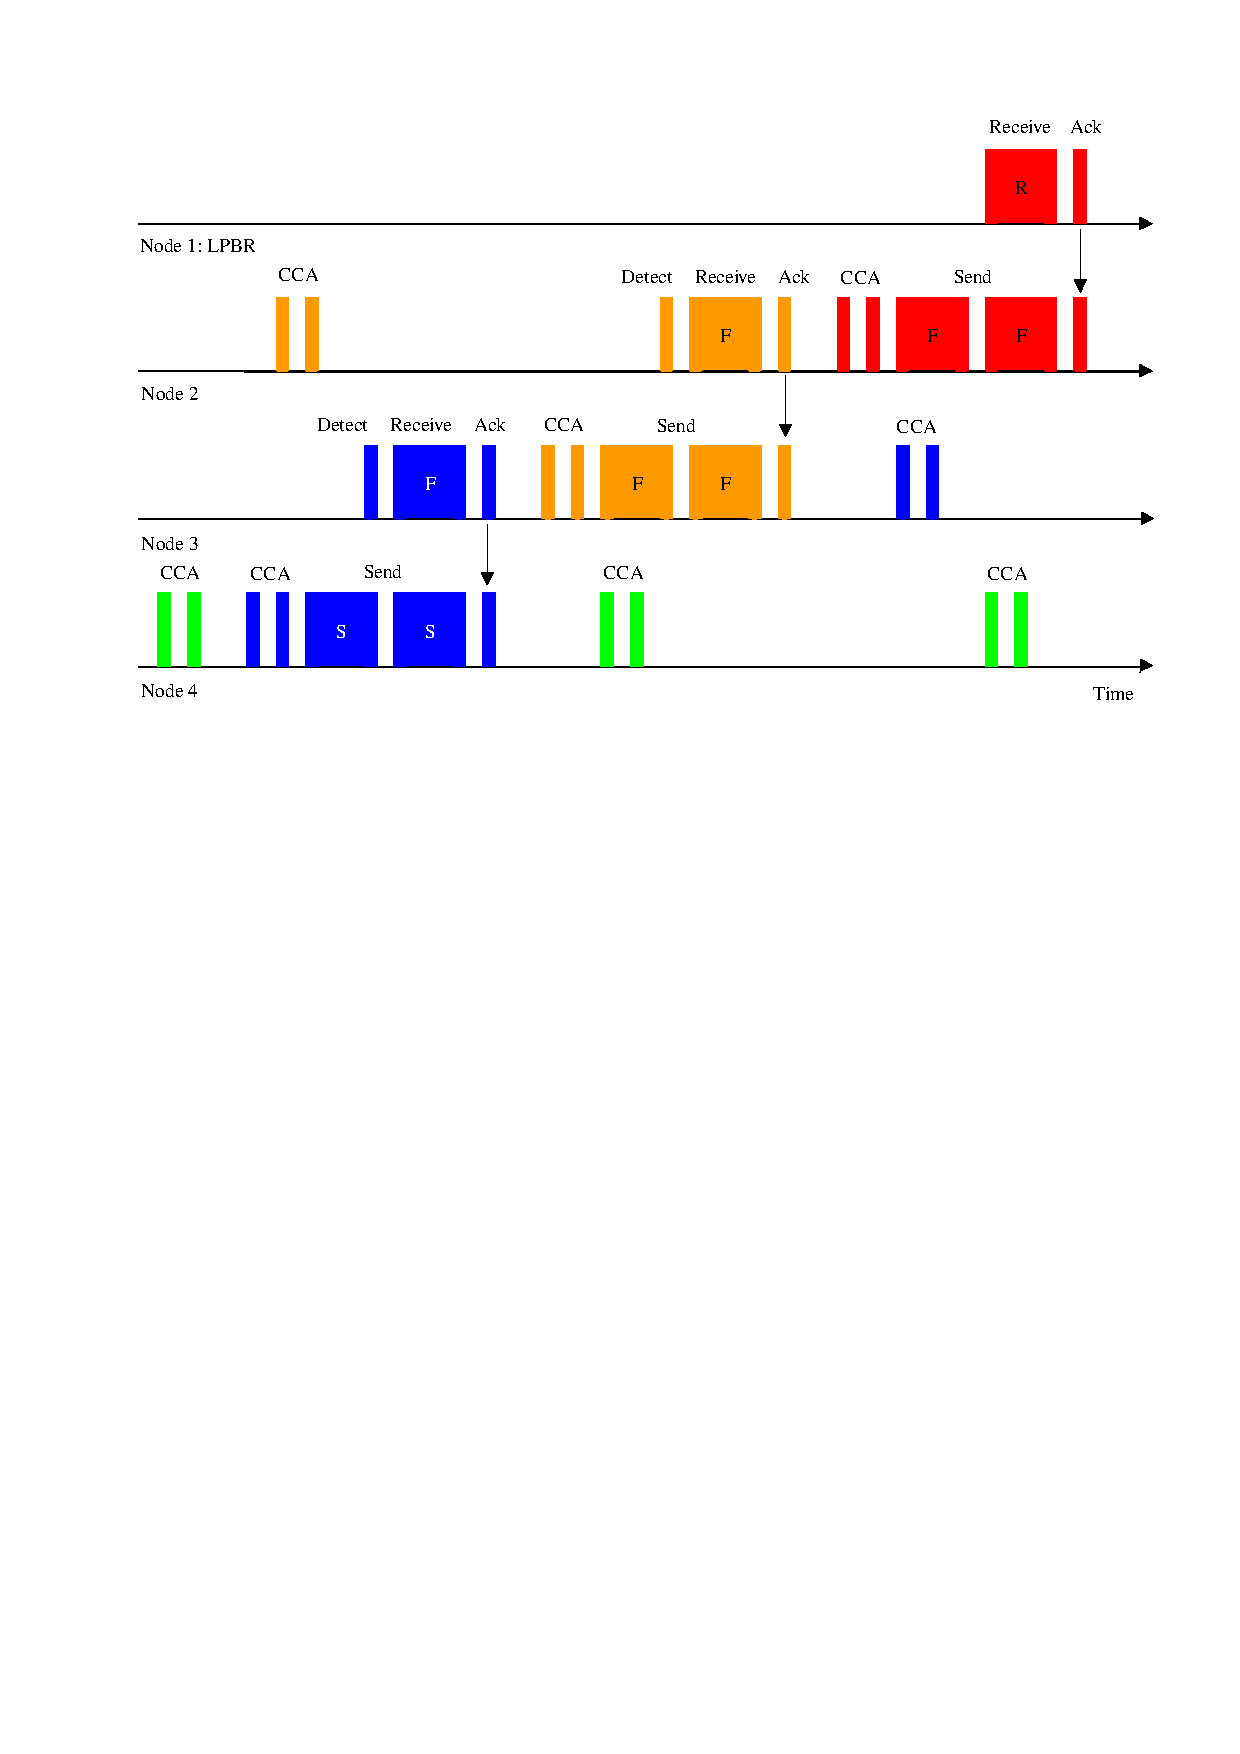
\includegraphics[trim=2cm 17cm 1cm 2cm, clip=true, totalheight=0.35\textheight]{mcrp2.pdf}
%\caption{Multichannel ContikiMAC multi hop packet transmission}
%\label{fig_mac}
%\end{figure}

Figure \ref{mcrptx} shows an example of a multi hop packet transmission in MCRP. The different colours represent different channels. Node 4's channel is represented by green, node 3 is blue, node 2 is yellow and node 1 is red. At each hop, the node changes to the next hop listening channel as shown in Figure \ref{fig_mcrpTopology} before forwarding the packet. Figure \ref{fig_mac} shows the transmission processes which includes the wake ups and transmission (forwarding) channel change that happens from node 4 (the sender) to node 1 which is the LPBR. \textit{R} represents receiving packet, \textit{F} is forwarding packet and \textit{S} is sending packet. 

The example in Figure \ref{mcrptx} shows node 4 is sending a packet to node 1, the LPBR through node 3 and node 2. Node 4 wakes up and checks for incoming packets on its channel. As it has a packet to be sent to node 1, it checks the next hop channel which is node 3 and changes the channel to node 3 listening channel (blue). It checks if the channel is clear for transmission using CCA. The CCA relies on the RSSI threshold to detect the radio activity on the channel. The CCA returns a positive value to indicate that the channel is clear and proceed to send the packet to node 3 on node 3 channel. Node 3 detects the packet when it wakes up and receives the packet. Node 3 sends the link layer acknowledgement to node 4 so that node 4 stops sending the packet. Node 4 goes back to sleep and wake ups at the next cycle on its channel (green) to check for any incoming or outgoing message for the node. If there is none, the node goes back to sleep. As node 3 is not the destination, it forwards the packet to node 2 on node 2 channel and node 2 to node 1, the LPBR which is the destination node. All nodes reset their channel after the transmission and wake up on their own listening channel.

\begin{figure}[H]
\centering

\subfigure[Topology diagram]{
\label{fig_mcrpTopology}
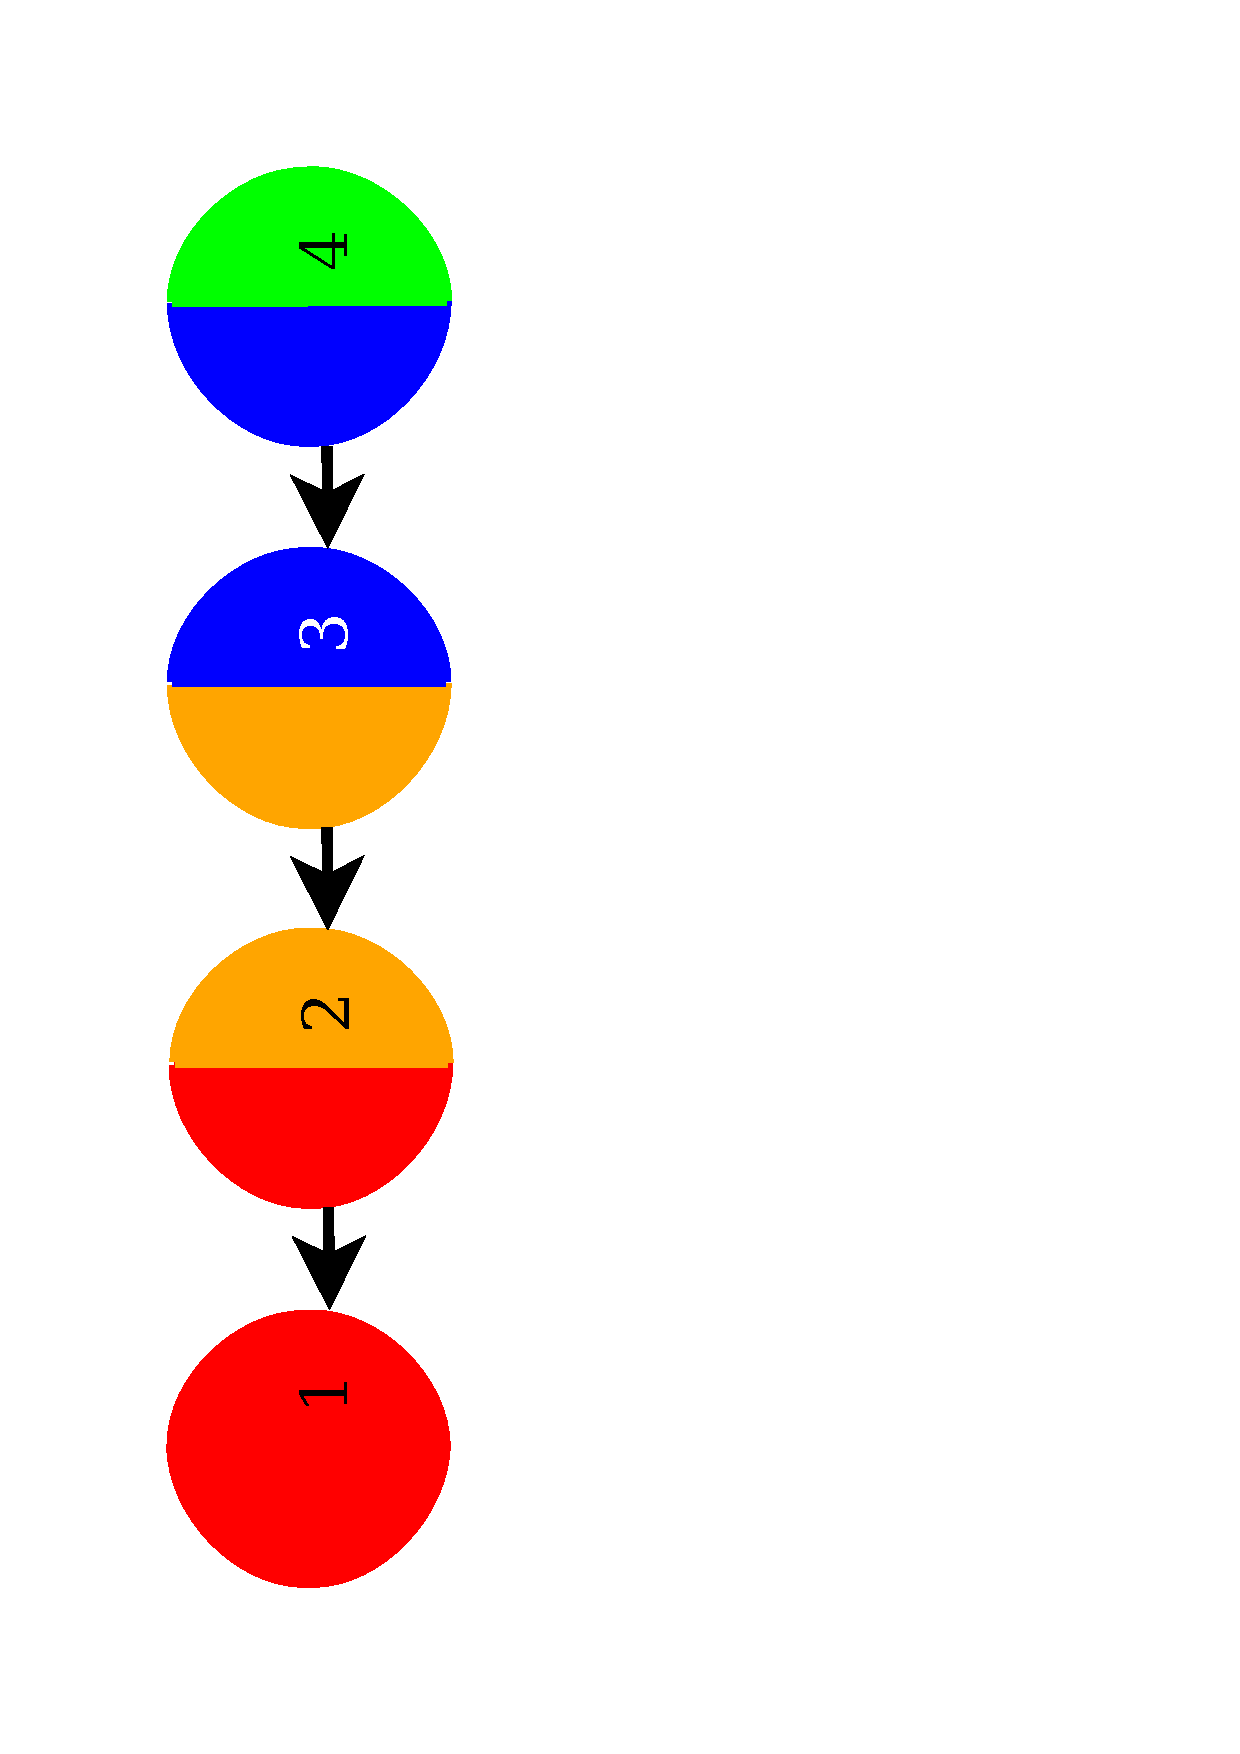
\includegraphics[trim=2cm 2cm 10cm 2cm, angle=270, clip=true, totalheight=0.10\textheight]{mcrpTopology2.pdf}
%\caption{Multichannel ContikiMAC multi hop packet transmission}
 }

\subfigure[Transmission channels]{
\label{fig_mac}
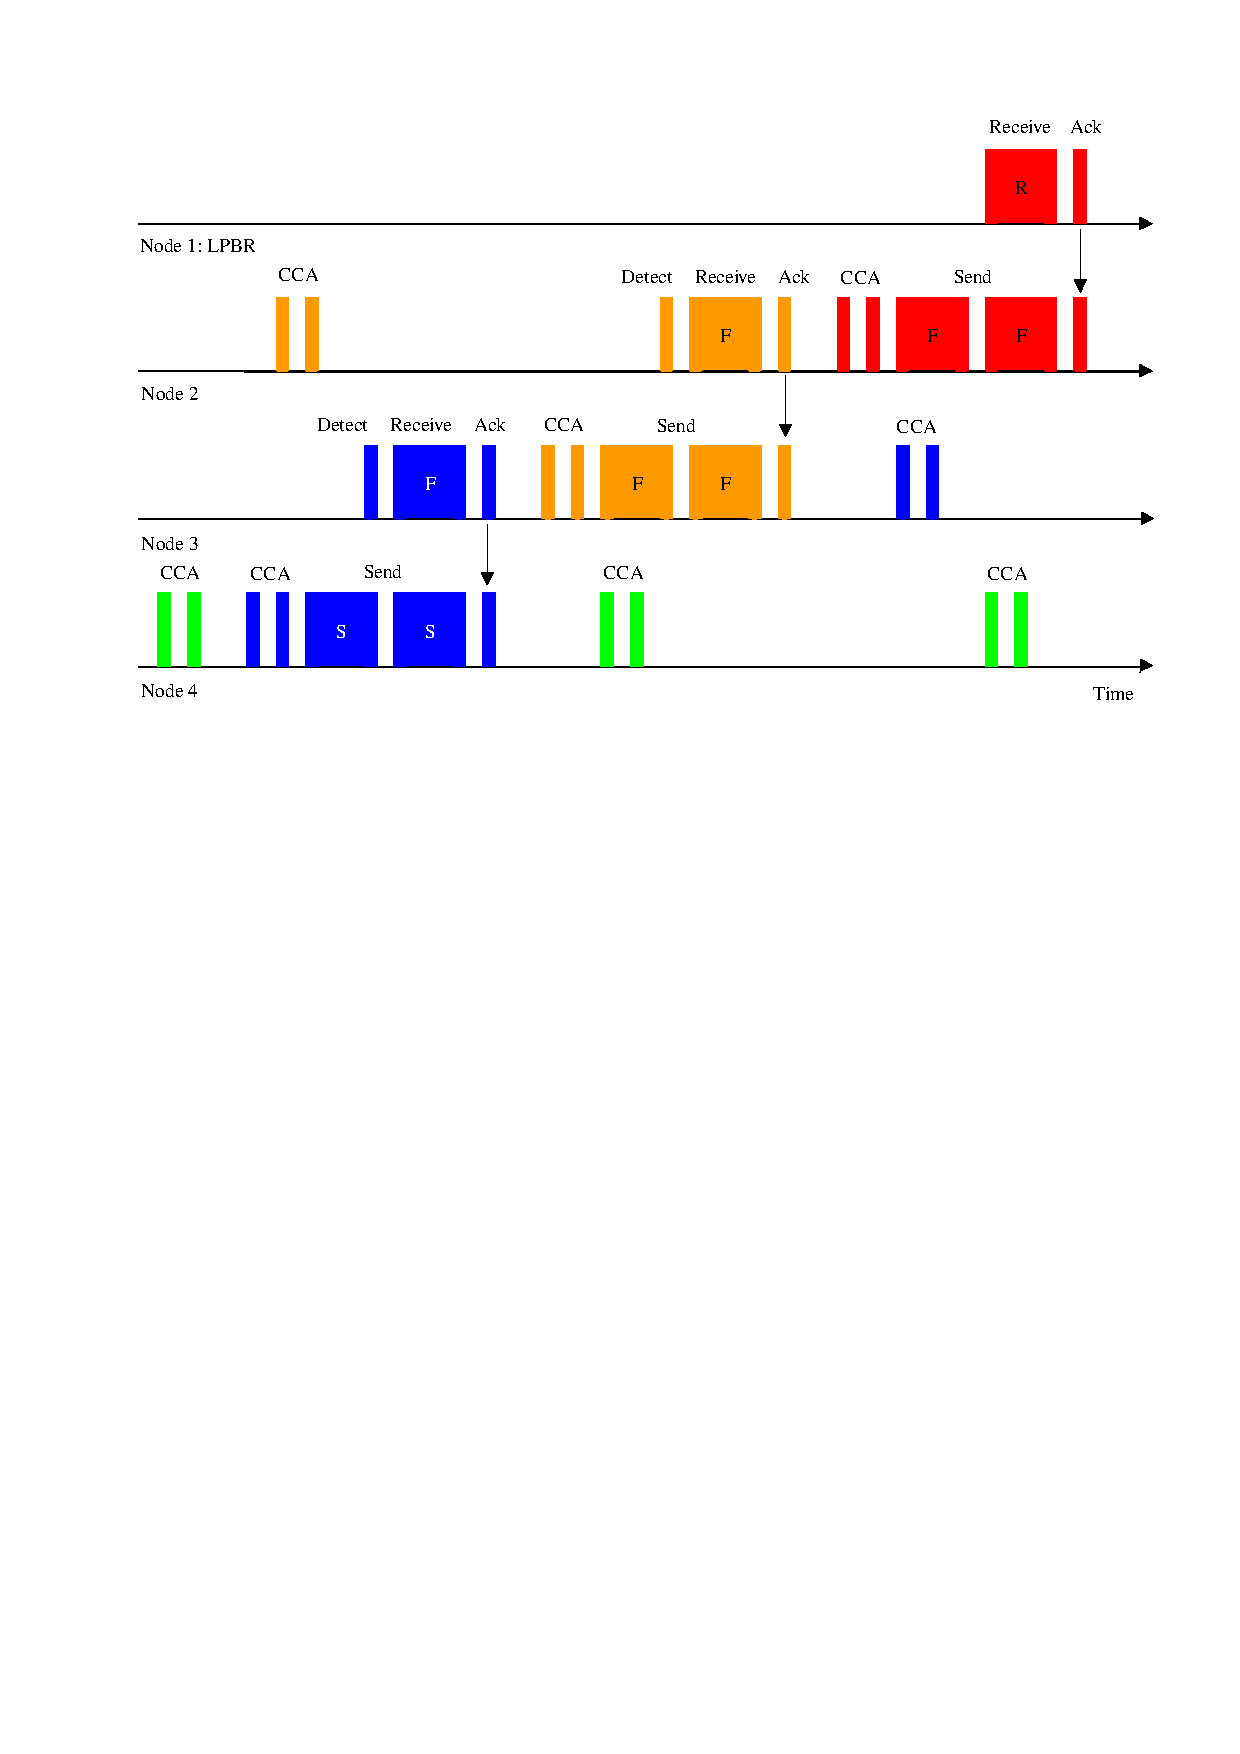
\includegraphics[trim=2cm 17cm 1cm 2cm, clip=true, totalheight=0.35\textheight]{mcrp2.pdf}
%\caption{Multichannel ContikiMAC multi hop packet transmission}
 }
\caption{MCRP multi hop packet transmission}
\label{mcrptx}
\end{figure}

%If the node has a packet to send, it needs to access the neighbour channel to be able to transmit a packet on the correct channel. 

%ContikiMAC has retransmitted, collisions valued. These values are used in probing to decide on the channel condition. These values are passed to the application layer to decide on channel change. The packet can be retransmitted for ( ) times before it is dropped. However, if the channel is busy, and the packet has not been sent (collisions before sending), it can stay in the loop for a long time.

%//////It uses (EXPLAIN CONTIKIMAC - refer to contikimac paper; why it's good, how it works). Also about retransmission and buffers. (maybe at next section???) 
%The transmitting channel is set at the MAC layer as packets are not send immediately if there are packets being queued. 
%The channel is reset to the transmitting channel before it tries to send and it is then reset to the listening channel to wait and listen to any packets that is being sent to the node. 

%The default ContikiMAC is a single channel protocol. It is modified to be able to work with multi channel nodes while (stick/hold/is) on the same principle of a low power ContikiMAC (minor changes to support multi channel without changing the main purpose of ContikiMAC).//////

\subsection{Network Layer}
%///net/rpl/rpl-icmp6.c and rpl-timers.c - the changes done!!

RPL is explained in Section \ref{routingProtocols}. RPL control messages are tailored to accommodate MCRP proposal. Two main changes to RPL control messages are the DIS (which is sent by a new node to make it possible for a node to require DIO messages from a reachable neighbour) and DIO (the main source of routing control information) control messages. DIS and DIO control messages are usually sent using broadcast. However, DIS and DIO support unicast. MCRP sends RPL DIS control message in broadcast and DIO in both broadcast and unicast. 

In MCRP, a new node that would like to join an existing tree needs to send the DIS control message to the reachable neighbours. However, as the reachable neighbours could be on different channel than it were initially during start up, the new node needs to send the DIS message on all channels available to be able to find the neighbours. 

The neighbours that receive the DIS message will reply with a DIO message and a packet that tells the new node of its channel to communicate on. The new node updated the neighbour table and has successfully joined the tree. 

If the neighbours do not receive the DIS from the new node before it is due to send the DIO message, the neighbours send a broadcast DIO on the default channel. The new node upon receiving the DIO will join the tree and updates the neighbour table. All neighbours send a DIO broadcast on the default channel and a DIO unicast for known neighbours on channels that the neighbours are listening on. 

One of the main reasons for this is because broadcasting on all channels would require more energy and it would take a longer time before all reachable nodes receive the control message. This could delay changes that might happen in the tree, i.e. changing of parent node. Secondly, all nodes by default will switch on to the same default channel as that is how the nodes are being set up. 

%Two RPL control messages that are changed are the DIO (which contains the routing control information) and DIS (to reach the neighbour) messages. 
%DIO is usually sent using broadcast. However, it is able to support unicast. MCRP sends RPL DIO control message in both broadcast and unicast. The DIO is sent as a broadcast in the default channel, which in this experiment is channel 26. The DIO is also sent as a unicast to the known neighbours 


%by enabling unicast to know the neighbours and broadcast to detect new nodes to join the tree.

%RPL is used as the routing protocol. (explain how RPL works briefly since it's explained in LITERATURE REVIEW).

%We tailored RPL control messages to be able to accommodate MRCP proposal by enabling unicast to know neighbours and broadcast to detect new nodes to join the tree.  

%////DIO UNICAST
%RPL sends the control messages as broadcast. However, as we are now dealing with multi channels, using broadcast for all channels would waste the bandwidth and costly as it would take a longer time to go through all channels. It would also cause congestion and the node to be on the broadcast channel and not ready on it's listening channel to be able to receive any incoming packets as it has not finish with the control message broadcast. RPL DIO message is able to deal with either broadcast or unicast. By default, broadcast was used as RPL is usually used with a single channel MAC. We enable the unicast DIO.

%////MULTI CHANNEL DIS
%If a new node tries to join the tree, it will send a DIS message on all channels until it finds the neighbours. 

%While this is true in the experiment, this might not be the case in the real world where the nodes could start at any channel. 
%We are looking into ways to overcome this problem.

%\section{Memory Footprint/Setup Overhead?}
%-how many packets more than usual?
%-memory consumption?